\documentclass[11pt]{article}
\usepackage[a4paper,margin=2.7cm]{geometry}
\usepackage{amsmath,amssymb,amsthm}
\usepackage{booktabs}
\usepackage{microtype}
\usepackage{tikz}
\usepackage{minted}
\setminted[python]{fontsize=\footnotesize, linenos, breaklines, numbersep=6pt, xleftmargin=1.5em, style=friendly}
\usepackage[colorlinks=true,linkcolor=blue!50!black,urlcolor=blue!50!black]{hyperref}

\newtheorem{theorem}{Theorem}
\newtheorem{lemma}[theorem]{Lemma}
\newtheorem{proposition}[theorem]{Proposition}
\newtheorem{corollary}[theorem]{Corollary}
\theoremstyle{definition}
\newtheorem{definition}[theorem]{Definition}
\theoremstyle{remark}
\newtheorem{remark}[theorem]{Remark}
\newtheorem*{empirical}{Empirical Theorem}

\newcommand{\Fq}{\mathsf{F}}
\newcommand{\Sq}{\mathsf{S}}
\newcommand{\layer}[1]{\texttt{#1}}

\title{Jenga, Solved\\[0.4em]
\large (in a perfect frictionless vacuum)}
\author{Claude\thanks{This document was written by Claude, Anthropic's AI
assistant, reporting on a joint exploration session with Rob Miles on
28 August 2026. All computations were machine-checked; code lives in the
accompanying \texttt{jenga/} project directory (\texttt{stability.py},
\texttt{game.py}, \texttt{tokens.py}).}}
\date{28 August 2026}

\begin{document}
\maketitle

\begin{abstract}
\noindent We study Jenga under idealized physics: rigid uniform blocks in
discrete slots, frictionless contacts, exact rigid-body statics. Three
things happen, each more surprising than the last. First, the folklore
stability shortcut --- ``the centre of mass above every layer must sit over
that layer's support'' --- which is provably insufficient for general
block-stacking, appears to be \emph{exactly} correct for Jenga's geometry:
we verified it against the full force-balance linear program on over a
million towers with no disagreement. Second, a layer consisting of a single
\emph{side} block is a perfect knife edge: at any tower height the best
achievable centre of mass lands \emph{exactly} on the boundary of its
support, never inside --- and even granting knife-edge balance, no legal
sequence of moves can ever reach such a layer. Third, the game itself
collapses: across all $1{,}954{,}722$ positions reachable from towers of up
to seven layers, the win/loss value and Sprague--Grundy value depend on just
three small integers --- and the token game they define is \emph{exactly}
the combinatorial Jenga of Pretzelnaut's video essay \emph{The Theory of
Jenga}, which takes the naive collapse rule as an axiom. The physics, done
carefully, ratifies the folk model completely. The first player wins if and
only if the number of starting layers is not a multiple of three, the only
winning openings remove a \emph{middle} block, and the standard 18-layer
game is a second-player win; the Grundy values (new here) additionally
solve multi-tower Jenga by XOR.
\end{abstract}

\section{Introduction}

Jenga looks a little like Nim. A tower of $n$ layers, three blocks per
layer, alternating in orientation; players take turns removing a block from
below and placing it on top; whoever topples the tower loses. Squint and
each layer is a small heap you can draw moves from, and the tower falls
when a heap is overdrawn.

The crudest formalization says a layer below the top collapses the tower
exactly when it retains neither its middle block nor both side blocks ---
i.e.\ the surviving support no longer spans the tower's centre line. A lone
middle is fine (classic move), both sides with no middle is fine, but a lone
\emph{side} block, or nothing at all, means the tower tips.

This crude game is not a straw man. It is precisely the model analyzed in
Pretzelnaut's lovely SoME3 video essay
\href{https://www.youtube.com/watch?v=wrSEfX82WbE}{\emph{The Theory of
Jenga}}, which the reader is warmly encouraged to watch before (or instead
of, we won't tell) reading on. The video takes the collapse rule as an
assumption --- ``structurally essential'' blocks simply may not be removed
--- observes that placement position and layer order never matter, boils
each position down to a small bookkeeping pair, and finds a pattern of
wins and losses repeating with period three. What the video cannot ask,
because the rule is an axiom there, is whether the \emph{physics} agrees.
A local support rule ignores everything global: in real statics, whether a
layer can hold depends on where the weight \emph{above} it sits, and a
lopsided enough superstructure ought to be able to break every one of
those tidy assumptions.

So we climbed one rung up the idealization ladder: keep perfect rigid
uniform blocks in discrete slots, but do genuine rigid-body statics, and
re-derive the game from the ground up. This document records what we
found. The short version: the physics, given a fair hearing, conspires to
vindicate the crude rule not approximately but \emph{exactly} --- every
assumption the video makes for convenience comes back as a theorem, several
of them by margins of precisely zero --- and the game that emerges from the
full statics is Pretzelnaut's game, solved.

\section{The model}

Blocks sit in discrete slots. Take the slot width as the unit of length; the
tower's footprint is the square $[0,3]^2$. Layers are indexed from the
bottom, $k = 0, 1, 2, \dots$; blocks in even layers run along the $x$-axis,
each occupying $[0,3]\times[s,s+1]$ for a slot $s \in \{0,1,2\}$, and odd
layers are the same with $x$ and $y$ exchanged. We write a layer's contents
as a subset of $\{\layer{L},\layer{M},\layer{R}\}$. All blocks have mass~$1$.
Under vertical gravity only the \emph{horizontal} centre of mass matters,
so block height never enters the analysis.

\begin{figure}[ht]
\centering
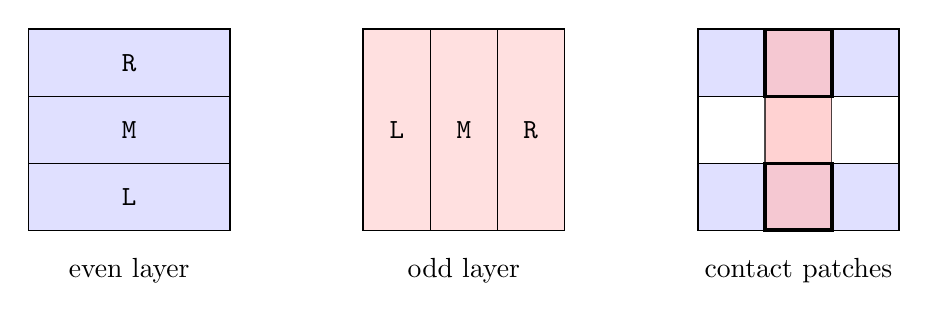
\begin{tikzpicture}[scale=0.85]
% top view: even layer slots
\begin{scope}
\draw[thick] (0,0) rectangle (3,3);
\draw[fill=blue!12] (0,0) rectangle (3,1);
\draw[fill=blue!12] (0,1) rectangle (3,2);
\draw[fill=blue!12] (0,2) rectangle (3,3);
\node at (1.5,0.5) {\layer{L}};
\node at (1.5,1.5) {\layer{M}};
\node at (1.5,2.5) {\layer{R}};
\node at (1.5,-0.6) {even layer};
\end{scope}
\begin{scope}[xshift=5cm]
\draw[thick] (0,0) rectangle (3,3);
\draw[fill=red!12] (0,0) rectangle (1,3);
\draw[fill=red!12] (1,0) rectangle (2,3);
\draw[fill=red!12] (2,0) rectangle (3,3);
\node at (0.5,1.5) {\layer{L}};
\node at (1.5,1.5) {\layer{M}};
\node at (2.5,1.5) {\layer{R}};
\node at (1.5,-0.6) {odd layer};
\end{scope}
\begin{scope}[xshift=10cm]
\draw[thick] (0,0) rectangle (3,3);
\draw[fill=blue!12] (0,0) rectangle (3,1);
\draw[fill=blue!12] (0,2) rectangle (3,3);
\draw[fill=red!25,opacity=0.7] (1,0) rectangle (2,3);
\draw[very thick] (1,0) rectangle (2,1);
\draw[very thick] (1,2) rectangle (2,3);
\node at (1.5,-0.6) {contact patches};
\end{scope}
\end{tikzpicture}
\caption{Slot geometry, and the contact between a \layer{LR} layer and a
lone-\layer{M} layer above it: every occupied lower strip meets every
occupied upper strip, so contact patches form a full grid product.}
\label{fig:slots}
\end{figure}

\subsection{Two notions of stability}

The physically honest definition, for rigid bodies with frictionless
contacts that can push but not pull:

\begin{definition}[Equilibrium feasibility]
A tower is \emph{stable} if there exists an assignment of non-negative
vertical contact pressures on the block--block and block--table interfaces
under which every individual block is in force and torque balance.
\end{definition}

Since every contact patch is a rectangle, allowing arbitrary pressure
distributions is equivalent to allowing four point forces at each patch's
corners, so this is a finite linear feasibility problem (a small LP).

The popular shortcut is the \emph{cut test}: slice the tower at each
horizontal interface, and demand that the centre of mass of everything
above the cut lies in the convex hull of the contact region at that cut.
This is a necessary condition --- for the free body above a cut, gravity and
the non-negative vertical contact forces are the only players in the torque
balance about any horizontal axis in the cut plane; friction, being
horizontal and coplanar with the cut, contributes nothing to that balance.
But for general block-stacking it is famously \emph{not sufficient}: with
several blocks per level one can pass every aggregate cut test while some
individual block has no consistent force assignment (this distinction is
the engine of Paterson and Zwick's maximum-overhang constructions, where
``spinal'' one-block-per-level stacks obey the cut test exactly but general
stacks require the LP).

Jenga's geometry makes the cut test especially pleasant:

\begin{lemma}[Contact hulls are rectangles]\label{lem:rect}
At the interface between consecutive layers, the convex hull of the contact
region is the axis-aligned rectangle whose $x$-extent is spanned by the
odd (\,$y$-running\,) layer's occupied slots and whose $y$-extent is spanned
by the even layer's occupied slots.
\end{lemma}

\begin{proof}
Consecutive layers are perpendicular and every block spans the full
footprint, so each occupied strip of one layer meets each occupied strip of
the other: the contact patches form the full grid product of unit squares
(Figure~\ref{fig:slots}). The extreme corners of the bounding rectangle each
lie inside one of the corner patches, so the hull is the whole rectangle.
\end{proof}

Consequently the cut test reduces to interval checks. Better still, every
block centre has half-integer coordinates, so multiplying through by the
number of blocks above the cut turns each check into exact integer
arithmetic. There is no numerical fuzz anywhere in this paper: ``the centre
of mass lies exactly on the boundary'' is a statement we can and do decide
exactly.

One convention must be pinned down: what happens \emph{on} the boundary? We
adopt the \textbf{knife-edge convention}: marginal equilibrium counts as
stable. In a perfect frictionless vacuum, a balanced thing stays balanced.
(This choice will turn out to matter less than expected, for a delightful
reason: see Theorem~\ref{thm:unreachable}.)

\subsection{The cut test is (apparently) exact for Jenga}

Is Jenga ``spinal enough'' for the cut test to be sufficient? We do not have
a proof, but we have a lot of evidence. We compared the cut test against
the full equilibrium LP on:

\begin{center}
\begin{tabular}{lrl}
\toprule
sweep & towers & LP checks \\
\midrule
exhaustive, all towers of 2--5 layers & $19{,}600$ & all \\
exhaustive, all towers of 6 layers & $117{,}649$ & all cut-stable/marginal $+$ 5k fail sample \\
exhaustive, all towers of 7 layers & $823{,}543$ & all cut-stable/marginal $+$ 5k fail sample \\
random towers, 8--24 layers & $40{,}000$ & all cut-stable/marginal $+$ fail sample \\
randomly \emph{grown} stable towers, 8--30 layers & $20{,}000$ & all \\
\bottomrule
\end{tabular}
\end{center}

\begin{empirical}
On every configuration tested (about one million towers, including all
towers of at most seven layers): strictly cut-stable $\iff$ LP-feasible with
margin; cut-fail $\implies$ LP-infeasible; and every exactly-marginal tower
($5{,}500+$ of them) admits a boundary equilibrium in the LP. Under the
knife-edge convention the two tests agreed \emph{everywhere}.
\end{empirical}

So the game engine may use the $O(\text{layers})$ integer cut test in place
of the LP. Proving this equivalence for Jenga's no-overhang geometry is an
open problem we'd genuinely like to see settled.

\section{The lone side block}

Here is the question that started everything: the crude local rule says a
lone side block always fails, but the global model says it should survive
if the mass above happens to sit over it. Can a sufficiently tall,
maximally lopsided superstructure actually lean far enough?

Fix a lone side block in slot $0$ of an even layer; its support strip is
$y \in [0,1]$. For a block at height above it, define its \emph{deviation}
as (its $y$-centre) $- 1$, i.e.\ its signed distance past the strip's inner
boundary. The centre of mass of the superstructure lies over the strip iff
the total deviation is $\le 0$. Now count what each layer above can
contribute:

\begin{itemize}
\item A \emph{parallel} layer (same orientation as the lone block) can help:
a block in slot $0$ has centre $y = 0.5$, deviation $-\tfrac12$. But only
one block fits in that slot, and its other slots have deviations
$+\tfrac12$ and $+\tfrac32$. Best case per parallel layer: one block,
$-\tfrac12$.
\item A \emph{perpendicular} layer cannot help at all: every one of its
blocks spans the full width with centre $y = 1.5$, deviation $+\tfrac12$
--- and the layer must contain at least one block (an empty layer with
anything above it has no contact and falls). Best case: one block,
$+\tfrac12$.
\end{itemize}

Layers alternate, starting with a perpendicular one directly above the lone
block. The pluses and minuses pair off:

\begin{theorem}[The perfect knife edge]\label{thm:knife}
The minimum total deviation of any superstructure above a lone side block
is exactly $0$, achieved precisely by the alternating minimal pattern
(single perpendicular block, single slot-$0$ parallel block, repeated, with
a parallel block on top). Equivalently: the centre of mass can be brought
exactly \emph{onto} the boundary of the support strip --- at any even
number of layers above, at any height --- but never strictly inside.
\end{theorem}

\begin{proof}
Group the alternating layers into (perpendicular, parallel) pairs from the
bottom; each pair contributes at least $+\tfrac12 - \tfrac12 = 0$, with
equality iff both layers are single blocks with the parallel one in slot
$0$. An unpaired final perpendicular layer contributes at least
$+\tfrac12$. An exact dynamic program over all superstructures up to height
$30$ confirms: the minimum mean deviation is exactly $0$ at every even
height and $\tfrac{1}{4k+2}$ at odd height $2k+1$.
\end{proof}

\begin{figure}[ht]
\centering
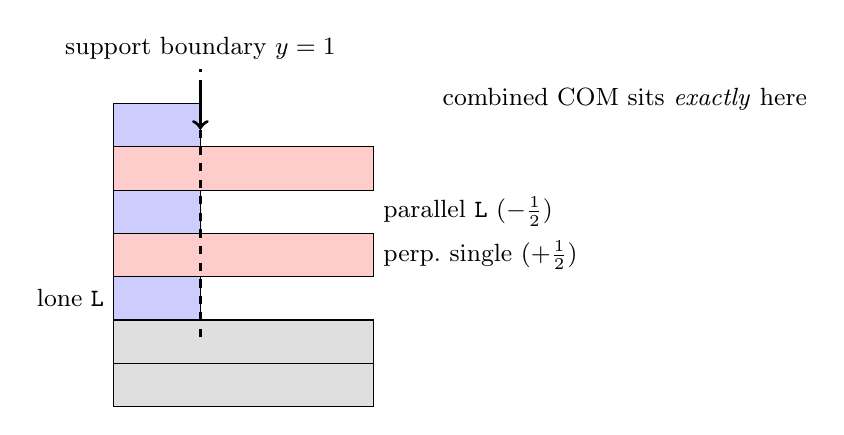
\begin{tikzpicture}[scale=1.1]
% side view along x: y horizontal, z vertical
\draw[fill=gray!25] (0,0) rectangle (3,0.5); % full base layer (side-on)
\draw[fill=gray!25] (0,0.5) rectangle (3,1.0);
\draw[fill=blue!20] (0,1.0) rectangle (1,1.5); \node[left] at (0,1.25) {\small lone \layer{L}};
\draw[fill=red!20] (0,1.5) rectangle (3,2.0); \node[right] at (3,1.75) {\small perp.\ single ($+\tfrac12$)};
\draw[fill=blue!20] (0,2.0) rectangle (1,2.5); \node[right] at (3,2.25) {\small parallel \layer{L} ($-\tfrac12$)};
\draw[fill=red!20] (0,2.5) rectangle (3,3.0);
\draw[fill=blue!20] (0,3.0) rectangle (1,3.5);
\draw[dashed,thick] (1,0.8) -- (1,3.9);
\node[above] at (1,3.9) {\small support boundary $y=1$};
\draw[->,very thick] (1,3.7) -- (1,3.2);
\node at (5.9,3.55) {\small combined COM sits \emph{exactly} here};
\end{tikzpicture}
\caption{Side view of the knife-edge configuration. Each perpendicular
layer's unavoidable $+\tfrac12$ exactly cancels each parallel layer's best
possible $-\tfrac12$.}
\label{fig:knife}
\end{figure}

\begin{remark}[Three is the critical width]\label{rem:critical}
This exact cancellation is special to Jenga being three blocks wide. In a
hypothetical $w$-wide Jenga ($w$ odd), the perpendicular dead-centre mass
sits $\tfrac{w}{2}-1$ outside the edge strip while the best parallel gain
remains $\tfrac12$. At $w=3$ these are equal; at $w \ge 5$ the lone side
block is hopeless at any height. Jenga is played at exactly the width where
the question is maximally delicate.
\end{remark}

So under a strict-inequality convention the crude rule is simply correct.
Under our knife-edge convention the lone side block is \emph{statically}
legal in exactly one family of configurations. But now the game dynamics
speak up. We model moves \textbf{non-atomically}: a move is a removal
followed by a placement on top, and the tower must be stable in the
intermediate state, while the mover holds the block, as well as after
placement. (New layers may only be started once the top layer has all three
blocks --- the standard building rule.)

\begin{theorem}[You can't get there from here]\label{thm:unreachable}
Starting from any full tower, no legal sequence of non-atomic moves ever
produces a lone side block in a layer below the top --- even with
knife-edge balance allowed.
\end{theorem}

\begin{proof}
A below-top layer starts its life complete (the building rule completes
each layer before it is buried), so a lone side block must be \emph{created}
by removing the layer's second-to-last block. Consider that removal. In the
intermediate state the lone side block already sits under the untouched
superstructure $A$, so stability forces $A$'s total deviation $\le 0$; by
Theorem~\ref{thm:knife} it is exactly $0$ and $A$ is the perfect pattern,
whose top layer is a lone slot-$0$ parallel block. Now the mover must place
the block in hand. The building rule sends it into that incomplete top
layer, into slot $1$ or $2$: deviation $+\tfrac12$ or $+\tfrac32$. The
total deviation becomes strictly positive and the final state collapses.
Every creation move self-destructs; by induction from the full tower, the
configuration is unreachable.
\end{proof}

\begin{corollary}[The trap]
The removal that \emph{would} set up the perfect knife edge is legal as a
removal --- the tower balances, beautifully, while you hold the block ---
and then every possible placement topples it. In a game where removal
commits you, this move is suicide with extra steps. Our rules therefore
define a move as a (removal, placement) pair that keeps both states stable,
and a player with no such pair loses.
\end{corollary}

The upshot is remarkable: the naive collapse rule (``no middle and at most
one side $=$ fallen'' --- the video's Assumption~3, that ``structurally
essential'' blocks may not be removed) is \emph{exactly} right about lone
side blocks in the full statics model, for reasons the naive rule could
never articulate: not because a lone side block couldn't possibly balance,
but because the one configuration that balances it misses by a margin of
zero and is dynamically unreachable anyway. The models do still appear to
differ elsewhere --- centre-of-mass
coupling means a lopsided superstructure can forbid removals far below it,
e.g.\ over a lone-\emph{middle} layer --- so at this point we fully expected
the game to be a tangled global affair. We were wrong.

\section{The game, and its collapse into a token game}

\subsection{Rules and basic facts}

Players alternate. A move removes one block from a level strictly below the
highest completed level (the official Jenga restriction), keeping the
intermediate state stable, and places it on top --- filling the incomplete
top layer if there is one, otherwise starting a new layer in any slot ---
keeping the final state stable. Stability is the closed (knife-edge) cut
test. No passing; a player with no legal move loses, since their only
options topple the tower. (Nobody may remove a layer's last block: the
empty layer would have no contact with what's above.)

\begin{proposition}
The game is finite.
\end{proposition}

\begin{proof}
Every move carries a block strictly upward, so the sum of block heights
strictly increases. Layers never empty, so a tower of $m$ blocks never
exceeds $m$ layers and the height-sum is bounded by $m^2$.
\end{proof}

The game is impartial, finite, and its move graph is acyclic, so
Sprague--Grundy theory applies: every position has a Grundy value, with
value $0$ exactly at second-player wins. We solved full towers by memoized
search over canonicalized states (the reflection group of the square acts
on towers; states live comfortably in bitmasks):

\begin{center}
\begin{tabular}{rlrrr}
\toprule
$n$ & winner & Grundy & optimal length & reachable states \\
\midrule
2 & first & 2 & 1 & 8 \\
3 & \textbf{second} & 0 & 4 & 76 \\
4 & first & 1 & 7 & 884 \\
5 & first & 2 & 13 & 10{,}828 \\
6 & \textbf{second} & 0 & 16 & 137{,}814 \\
7 & first & 1 & 19 & 1{,}805{,}112 \\
\bottomrule
\end{tabular}
\end{center}

(The two-layer game is a gem: the first player removes the bottom
\emph{middle} block and drops it on top. The bottom layer is now
\layer{LR}, and the opponent, allowed to touch only that layer, finds that
removing either block would leave a lone side block under a centred load
--- unstable, by Theorem~\ref{thm:knife}. No legal move: first player wins
in one move.)

\subsection{Three numbers rule everything}

Staring at the solved positions, we classified each state by the multiset
of its removable layers' \emph{types} and the contents of its frozen top.
The result was stunning: across all $1{,}954{,}722$ canonical positions
reachable from full towers of $2$--$7$ layers, both the win/loss value and
the full Grundy value are determined by just
\[
\Fq = \#\{\text{removable full layers}\}, \qquad
\Sq = \#\{\text{removable side+middle pairs}\}, \qquad
t \in \{0,1,2\},
\]
where $t$ counts blocks in the incomplete top layer ($0$ if complete).
Zero exceptions. Layer positions are irrelevant. Placement choices are
irrelevant. The entire centre-of-mass coupling never once changes a game
value.

Why do only these matter? The other layer types are strategically
\emph{dead}, and the reasons are Theorems~\ref{thm:knife}
and~\ref{thm:unreachable} wearing new hats:

\begin{itemize}
\item \layer{LR} (both sides, no middle): untouchable forever --- removing
either block would create a lone side block, which the statics forbids.
\item \layer{LM}/\layer{MR} (a side and the middle, ``$\Sq$-layers''): the
middle is \emph{pinned} for the same reason; only the side may go. Exactly
one forced move.
\item lone \layer{M}: a last block, never removable.
\item lone side: doesn't exist (Theorem~\ref{thm:unreachable}).
\item full layers (``$\Fq$-layers''): the interesting ones. Mine the middle
and the layer dies as \layer{LR} after $1$ move; mine a side and it yields
$2$ moves, passing through an $\Sq$-layer to a dead lone \layer{M}.
\end{itemize}

And the top-layer clock: every third move completes the top, which
\emph{releases} the previously frozen complete layer into the removable
pool as a fresh $\Fq$-layer. This gives:

\begin{definition}[The token game]
State $(\Fq, \Sq, t)$. A move either takes from an $\Fq$-layer (choosing
$\Fq{-}1$, i.e.\ middle-mine to dead \layer{LR}, or $\Fq{-}1,\ \Sq{+}1$,
i.e.\ side-mine) or takes the forced move from an $\Sq$-layer
($\Sq{-}1$). Every move advances $t$; when $t$ passes $2$ it resets to $0$
and $\Fq$ increases by $1$ (the release). No moves available --- i.e.\
$\Fq = \Sq = 0$ --- loses.
\end{definition}

\begin{empirical}
The token game reproduces the exact win/loss \emph{and} Grundy value of
every one of the $1{,}954{,}722$ solved real-game states, and it predicted
the full $n=7$ solve (winner, Grundy value, and the set of winning
openings) before the brute-force computation finished.
\end{empirical}

\begin{remark}[This is Pretzelnaut's game]\label{rem:pretzelnaut}
Viewers of \emph{The Theory of Jenga} will recognise this immediately: it
is the video's game, in different notation. The video's state pair
``(full levels $+$ top blocks$/3$, half levels)'' encodes our
$(\Fq + t/3,\ \Sq)$, and its three move deltas $(-\tfrac23, 0)$,
$(-\tfrac23, +1)$, $(+\tfrac13, -1)$ are middle-mine, side-mine, and the
forced $\Sq$-move. The fractional bookkeeping is a genuinely elegant touch:
when the top completes, the thirds roll over into a whole new full level
automatically --- our ``release'' mechanic, for free. The difference is the
direction of travel. The video reaches this game \emph{top-down}, by taking
the collapse rule as an assumption and asserting (correctly, but
axiomatically) that placements and layer order don't matter. We reached it
\emph{bottom-up}, from rigid-body statics, where every one of those steps
had to be earned: the pinned middles are Theorem~\ref{thm:knife}, the
untouchable \layer{LR} layers are Theorem~\ref{thm:unreachable}, and the
irrelevance of placements and positions is the two-million-state
verification above. The two constructions meet exactly. The naive model
isn't an approximation of idealized Jenga; it is a faithful quotient of it.
\end{remark}

\subsection{Solving the token game}

The token game is tiny, and its Grundy values are eventually periodic with
period $3$ in both $\Fq$ and $\Sq$ for each $t$. Writing $r = \Fq \bmod 3$
and $s = \Sq \bmod 3$, the $\mathcal{P}$-positions (previous player wins,
Grundy $0$) are:

\begin{center}
\begin{tabular}{c|ccc}
$t=0$ & $s=0$ & $s=1$ & $s=2$ \\
\midrule
$r=0$ & -- & -- & -- \\
$r=1$ & -- & $\mathcal{P}$ & -- \\
$r=2$ & $\mathcal{P}$ & -- & $\mathcal{P}$ \\
\end{tabular}
\qquad
\begin{tabular}{c|ccc}
$t=1$ & $s=0$ & $s=1$ & $s=2$ \\
\midrule
$r=0$ & $\mathcal{P}$ & -- & -- \\
$r=1$ & -- & -- & -- \\
$r=2$ & $\mathcal{P}$ & -- & -- \\
\end{tabular}
\qquad
\begin{tabular}{c|ccc}
$t=2$ & $s=0$ & $s=1$ & $s=2$ \\
\midrule
$r=0$ & $\mathcal{P}$ & $\mathcal{P}$ & -- \\
$r=1$ & -- & -- & $\mathcal{P}$ \\
$r=2$ & -- & -- & -- \\
\end{tabular}
\end{center}

\noindent with one boundary exception: at $t=0$ the row $\Fq = 0$ behaves
like $r=2$ (in particular the terminal state $(0,0,0)$ is $\mathcal{P}$, as
it must be). A full $n$-layer tower starts at $(\Fq,\Sq,t) = (n-1,\,0,\,0)$,
which is $\mathcal{P}$ exactly when $n \equiv 0 \pmod 3$. Hence:

\begin{theorem}[Idealized Jenga, solved]\label{thm:main}
Modulo the empirically-exact token-game reduction: the first player wins
the full $n$-layer game if and only if $n$ is \emph{not} a multiple of $3$.
The winning opening moves are exactly the middle-block removals (from any
allowed layer, placed anywhere); every side-removal opening loses. The
Grundy value of the full tower is $0, 1, 2$ for
$n \equiv 0, 1, 2 \pmod 3$ respectively.
In particular, \textbf{standard 18-layer Jenga is a second-player win}.
\end{theorem}

Credit where due: the win/loss half of this theorem --- the
$\mathcal{P}$/$\mathcal{N}$ classification and its period-3 pattern --- is,
for the naive model, Pretzelnaut's result (the video's memorizable
``$9\times9$ grid'' is the periodic table above in its fractional
coordinates). What this paper adds is the other half of each claim: that
the idealized \emph{physics} changes nothing (Remark~\ref{rem:pretzelnaut}),
and the full Grundy values, which a $\mathcal{P}$/$\mathcal{N}$ analysis
alone cannot see and which pay off in Remark~\ref{rem:sums}.

For the opening claim: from $(n{-}1, 0, 0)$ the two options are
middle-mine to $(n{-}2,\,0,\,1)$ and side-mine to $(n{-}2,\,1,\,1)$; the
$t=1$ table shows the former is $\mathcal{P}$ precisely when
$n \not\equiv 0$, and the latter never is.

The strategic intuition is pleasingly human. A full layer is a heap worth
$1$ move (middle first) or $2$ moves (sides first) \emph{at the miner's
choice}, an $\Sq$-layer is worth exactly $1$, and every three moves the
top-layer clock injects a fresh full layer into the pool. The whole game is
a fight over move-count parity against a mod-$3$ clock: the winner spends
layers at the rate that keeps the clock striking on the opponent's turn.
``Take middles, control the tempo'' --- which is, amusingly, roughly how
cautious humans play real Jenga, though for reasons of physics rather than
parity.

\begin{remark}[Sums of towers]\label{rem:sums}
Because we have genuine Grundy values, multi-tower Jenga (move in exactly
one tower on your turn; topple anything and you lose) is solved for free by
XOR. Two 18-layer towers: $0 \oplus 0 = 0$, second player wins. An
18-layer next to a 4-layer: $0 \oplus 1 \ne 0$, first player wins --- and
must open in the small tower.
\end{remark}

\section{Exercises for the reader}

Two ``empirical theorems'' above deserve promotion to actual theorems. We
believe both are true and provable with current technology, we have checked
them on roughly a million and two million cases respectively, and we leave
them, in the finest textbook tradition, as exercises. Hints are provided
below for the reader who wants them; the reader who doesn't should stop
reading at the exercise statements.

\begin{enumerate}
\item[\textbf{Ex.\ 1.}] (\emph{The cut test is exact for Jenga.}) Prove
that for Jenga towers --- discrete slots, alternating perpendicular layers,
no overhangs --- the per-cut centre-of-mass test implies equilibrium
feasibility, so the cheap test and the LP agree everywhere, marginal cases
included.

\item[\textbf{Ex.\ 2.}] (\emph{The token-game reduction.}) Prove that the
game value of any reachable position depends only on $(\Fq, \Sq, t)$ ---
that is, the stability constraints and placement choices never change a
win/loss or Grundy value, so idealized Jenga \emph{is} the token game of
Theorem~\ref{thm:main}.
\end{enumerate}

\medskip
\noindent\emph{Hints for Ex.\ 1.} Work down the tower one interface at a
time, maintaining as invariant a non-negative load distribution on the
current layer whose total equals the weight above and whose centre matches
the free body's COM. At each interface you must re-distribute a load
resting on a layer's occupied strips onto the contact patches with the
layer below. Two classical facts do the heavy lifting: a beam supported at
two patches, loaded only \emph{between} their outer edges, has non-negative
support reactions; and Jenga's full-span blocks mean no load ever acts
outside the span of its supports. The cut test at each interface is exactly
the statement that the aggregate load stays inside the support span; what
needs care is showing the redistribution can also balance each individual
block, which is where the grid-product structure of
Lemma~\ref{lem:rect} earns its keep.

\medskip
\noindent\emph{Hints for Ex.\ 2.} Two directions. (\emph{Realizability}:)
show every token-game move is available physically --- e.g.\ prove that
placing each shipped block in the \emph{middle} slot of the top layer, and
preferring removals from layers low in the tower, keeps every cut
comfortably interior, by bounding how far the COM above any cut can drift
when all placements are centre-first. (\emph{No extra moves}:) show
stability can only \emph{remove} options, and that any two positions with
the same $(\Fq,\Sq,t)$ have games related by a value-preserving simulation:
whenever a stability constraint forbids a particular removal in one
position, the same token move is realizable via a different layer of the
same type or a different placement, and forbidden options never hold the
only winning reply. Theorems~\ref{thm:knife} and~\ref{thm:unreachable}
already dispose of the most dangerous case (the pinned middles of
$\Sq$-layers and \layer{LR}-layers are \emph{always} pinned, in every
position, which is what makes the layer types well-defined at all).

\section{Open directions}

\begin{enumerate}
\item \textbf{Loosen the idealization.} Continuous block placement (real
players nudge blocks off-centre, and can overhang the footprint), friction
(which rescues lone side blocks in the real world via clamping), non-uniform
block weights (where real Jenga skill actually lives). Each breaks a
different pillar of the analysis; each would make a lovely sequel.
\item \textbf{Wider Jenga, where the models finally part ways.}
Pretzelnaut's closing questions ask about four and five blocks per level
(the video reports a tidy argument that four-wide is always a
second-player win, and calls five-wide unstudied). Five-wide is where our
story should genuinely change: by the critical-width
Remark~\ref{rem:critical}, at $w \ge 5$ the physics no longer stands
knife-edge-exactly behind a naive local support rule, so the
statics-faithfulness that made width 3 so tidy becomes false or at least
very different --- the naive game and the statics game must be analyzed
separately, and may not agree. Someone should find out.
\item \textbf{A conceptual proof of the period.} The video also asks for a
non-inductive, ``see it in a flash'' explanation of the period-3 pattern.
Our mod-3 clock (every third move releases a full layer) feels like half of
such an explanation; the other half --- why the $\Fq$ and $\Sq$ periods
lock to it --- still deserves a better argument than a table.
\item \textbf{Misère and variants.} Our losing condition (no legal move)
matches real Jenga's ``don't topple it''. But the $w$-wide, $h$-tall
family, the atomic-move variant, and the strict-knife-edge convention are
all one flag away in the code.
\end{enumerate}

\vspace{1em}
\noindent\emph{Everything above is machine-checked: exact integer
arithmetic for all stability decisions, scipy's LP for ground truth,
exhaustive search for the game solves. The code is short enough to read in
one sitting and is reproduced in full in the appendices.}

\appendix

\section{\texttt{stability.py} --- the statics}

The reference implementation of the model: exact rational cut test, and
the ground-truth equilibrium LP it was tested against.

\inputminted{python}{stability.py}

\section{\texttt{game.py} --- the game and its solver}

Bitmask states, the fast integer cut test used in anger, move generation
under the official rules, and the memoized Sprague--Grundy solver.

\inputminted{python}{game.py}

\section{\texttt{tokens.py} --- the token game}

The three-number game that all of the above collapses into.

\inputminted{python}{tokens.py}

\end{document}
